%%%%%%%%%%%%%%%%%%%%%%%%%%%%%%%%%%%%%%%%%%%%%%%%%%%%%%%%%%
\frame {\frametitle{What is Apache Spark}
%%%%%%%%%%%%%%%%%%%%%%%%%%%%%%%%%%%%%%%%%%%%%%%%%%%%%%%%%%
\begin{itemize}
  \item Project goals:
  \begin{itemize}
    \item Generality: diverse workloads, operators, job sizes
    \item Low latency: sub-second
    \item Fault tolerance: faults are the norm, not the exception
    \item Simplicity: often comes from generality
  \end{itemize}
\end{itemize}

}

%%%%%%%%%%%%%%%%%%%%%%%%%%%%%%%%%%%%%%%%%%%%%%%%%%%%%%%%%%
\frame {\frametitle{Code Base (2012)}
%%%%%%%%%%%%%%%%%%%%%%%%%%%%%%%%%%%%%%%%%%%%%%%%%%%%%%%%%%
  \begin{figure}[h]
    \centering
    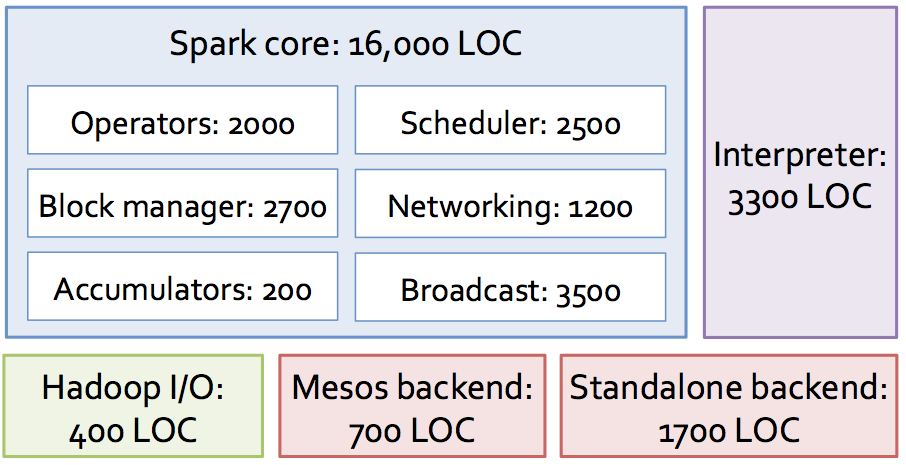
\includegraphics[scale=0.36]{./Figures/code_base}
    % \caption{Spark code base, as of 0.6.x (2012).}
    \label{fig:hdfs}
  \end{figure}

\begin{itemize}
  \item 2012 (version 0.6.x): 20,000 lines of code
  \item 2014 (branch-1.0): 50,000 lines of code
\end{itemize}
}


%%%%%%%%%%%%%%%%%%%%%%%%%%%%%%%%%%%%%%%%%%%%%%%%%%%%%%%%%%
\frame {\frametitle{Motivations}
%%%%%%%%%%%%%%%%%%%%%%%%%%%%%%%%%%%%%%%%%%%%%%%%%%%%%%%%%%
\begin{itemize}
  \item Software engineering point of view
  \begin{itemize}
    \item Hadoop code base is huge
    \item Contributions/Extensions to Hadoop are cumbersome
    \item Java-only hinders wide adoption, but Java support is fundamental
  \end{itemize}

  \item Data abstraction point of view
  \begin{itemize}
    \item New fundamental abstraction RDD
    \item Easy to extend with new operators
    \item More descriptive computing model
  \end{itemize}
  
  \item System/Framework point of view
  \begin{itemize}
    \item Simplified data flow
    \item Faster processing speed
    \item Unified pipeline
  \end{itemize}
\end{itemize}
}

%%%%%%%%%%%%%%%%%%%%%%%%%%%%%%%%%%%%%%%%%%%%%%%%%%%%%%%%%%
\frame {\frametitle{A More Descriptive Computing Model}
%%%%%%%%%%%%%%%%%%%%%%%%%%%%%%%%%%%%%%%%%%%%%%%%%%%%%%%%%%
\begin{itemize}
  \item WordCount in MR
  \item WordCount in Spark
  \item Transformations vs. Actions
\end{itemize}
}

%%%%%%%%%%%%%%%%%%%%%%%%%%%%%%%%%%%%%%%%%%%%%%%%%%%%%%%%%%
\frame {\frametitle{A Simplified Data Flow}
%%%%%%%%%%%%%%%%%%%%%%%%%%%%%%%%%%%%%%%%%%%%%%%%%%%%%%%%%%
\begin{itemize}
  \item Shows HDFS checkpointing
\end{itemize}
}

%%%%%%%%%%%%%%%%%%%%%%%%%%%%%%%%%%%%%%%%%%%%%%%%%%%%%%%%%%
\frame {\frametitle{Faster Processing Speed}
%%%%%%%%%%%%%%%%%%%%%%%%%%%%%%%%%%%%%%%%%%%%%%%%%%%%%%%%%%
\begin{itemize}
  \item PageRank example from nsdi paper (we know already pr)
  \item k-means example (Mapreduce vs Spark)
\end{itemize}
}

%%%%%%%%%%%%%%%%%%%%%%%%%%%%%%%%%%%%%%%%%%%%%%%%%%%%%%%%%%
\frame {\frametitle{Unified Pipeline}
%%%%%%%%%%%%%%%%%%%%%%%%%%%%%%%%%%%%%%%%%%%%%%%%%%%%%%%%%%
\begin{itemize}
  \item General diagram of spark and related components
\end{itemize}
}
